\documentclass[t]{beamer}
\usepackage[portuguese]{babel}
\usepackage[utf8]{inputenc}
\usetheme{Berkeley}
\usecolortheme{seahorse}

\addto\captionsportuguese{
	\renewcommand{\figurename}{Fig.}
	\renewcommand{\tablename}{Tab.}
}

\title{Micro-controladores}
\subtitle{Suas características principais e sua importância para a área de IoT.}

\AtBeginSection[]
{
	\begin{frame}
	\frametitle{Sumário}
	\tableofcontents[currentsection]
\end{frame}
}

\begin{document}

\frame{\titlepage}

\begin{frame}
\frametitle{Sumário}
\tableofcontents
\end{frame}

\section{Características}

\begin{frame}{O que é um micro-controlador?!}
\begin{itemize}
	\item Computador em um Chip
	\item Design embarcado
	\item Interrupções
	\item Clock
	\item Programável
\end{itemize}
\end{frame}

\section{Arquiteturas}

\begin{frame}{Arquiteturas}
\begin{itemize}
	\item Von Neumann
	\item Harvard
\end{itemize}
\end{frame}

\begin{frame}{Arquiteturas}
Von Neumann

\begin{figure}
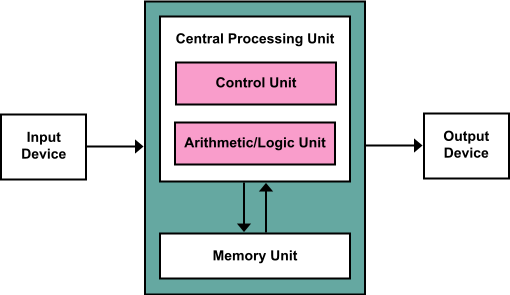
\includegraphics[width=\linewidth]{arquiteturavonneumann}
\end{figure}
\end{frame}

\begin{frame}{Arquiteturas}
Harvard

\begin{figure}
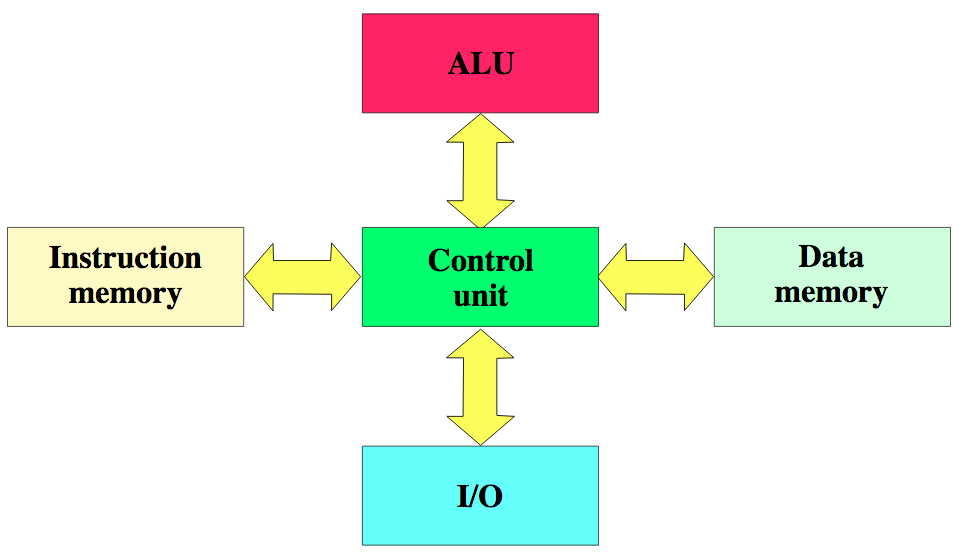
\includegraphics[width=\linewidth]{arquiteturaharvard}
\end{figure}
\end{frame}

\begin{frame}{Arquiteturas}
Conjuntos de Instruções
\begin{itemize}
\item CISC
\item RISC
\end{itemize}
\end{frame}

\section{Processadores}

\begin{frame}{Processadores}
Características
\begin{itemize}
	\item Clock
	\item BUS
	\item Memórias
	\item Arquiteturas
\end{itemize}
\end{frame}

\section{Memórias}

\begin{frame}{Memórias}
\begin{itemize}
	\item PROM (programmable read-only memory)
	\begin{itemize}
		\item EPROM
		\item EEPROM
		\item UV-EPROM
	\end{itemize}
	\item RAM
	\item ROM
	\item FLASH
\end{itemize}
\end{frame}

\section{Pinagem}

\begin{frame}{Pinagem}
\begin{itemize}
	\item Vin
	\item GND
	\item RST
	\item CLK
	\item RX
	\item TX
	\item GPIO
	\item I2C
\end{itemize}
\end{frame}

\section{Exemplos}

\begin{frame}{Exemplos}
\begin{itemize}
	\item Arduino
	\item Atmel AVR
	\item PIC (Microchip Technology)
\end{itemize}

\end{frame}


\frame{\titlepage}

\end{document}
